%Autor: Simon Walker
%Version: 1.0
%Datum: 28.04.2020
%Lizenz: CC BY-NC-SA

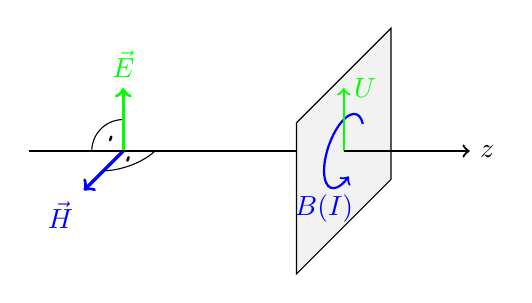
\begin{tikzpicture}[x={(0, 0.8cm)}, y={(-0.5cm,-0.5cm)}, z={(0.8cm, 0)}]

\def\l{7} %länge der z-Achse
\def\s{1.2} %Quadratgrösse (eine Seite ist s*2)
\def\p{5} %Positoon des Quadrates

\draw[domain=90:180,smooth,variable=\x] plot ({sin(\x)*0.5},{0}, {1.5+cos(\x)*0.5});
\draw[domain=0:90,smooth,variable=\x] plot ({0},{sin(\x)*0.5}, {1.5+cos(\x)*0.5});
\draw[fill=black] (0.2, 0, 1.3) circle[radius=0.03];
\draw[fill=black] (0, 0.2, 1.7) circle[radius=0.03];
\draw[very thick, green, ->] (0, 0, 1.5) -- (1, 0, 1.5) node[above, green] {$\vec{E}$};
\draw[very thick, blue, ->] (0, 0, 1.5) -- (0, 1, 1.5) node[below left, blue] {$\vec{H}$};

\draw[thick] (0, 0, 0) -- (0, 0, \p); %Beginn der Z-Achse

\draw[fill=gray!10] (-\s, -\s, \p) -- (-\s, \s, \p) -- (\s, \s, \p) -- (\s, -\s, \p) -- cycle;
\draw[->,domain=-75:195,smooth,variable=\x, blue, thick] plot ({cos(\x)*0.5},{sin(\x)*0.5}, {\p});
\node[blue] at (-0.6, 0.5, \p) {$B(I)$};
\draw[->, green, thick] (0, 0, \p) -- (1, 0, \p) node[right, green] {$U$};
\draw[thick, ->] (0, 0, \p) -- (0, 0, \l) node[right] {$z$}; %Ende der Z-Achse

\end{tikzpicture}
